\documentclass[10pt, compress, aspectratio=169]{beamer}

\usetheme[numbering=fraction, progressbar=none, titleformat=smallcaps]{metropolis}
\usepackage{booktabs}
\usepackage{array}
\usepackage{listings}
\usepackage{graphicx}
\usepackage[scale=2]{ccicons}
\usepackage{url}
\usepackage{relsize}
\usepackage{wasysym}

\usepackage{pgfplots}
\usepgfplotslibrary{dateplot}

\lstset{ %
  backgroundcolor={},
  basicstyle=\ttfamily\footnotesize,
  breakatwhitespace=true,
  breaklines=true,
  captionpos=n,
  commentstyle=\color{orange},
  escapeinside={\%*}{*)},
  extendedchars=true,
  frame=n,
  keywordstyle=\color{orange},
  language=bash,
  rulecolor=\color{black},
  showspaces=false,
  showstringspaces=false,
  showtabs=false,
  numbers=left,
  numbersep=3pt,
  stepnumber=1,
  stringstyle=\color{gray},
  tabsize=2,
  keywords={thrust,plus,device_vector, copy,transform,begin,end, copyin,
  copyout, acc, \_\_global\_\_, void, int, float, main, threadIdx, blockIdx,
  blockDim, if, else, malloc, NULL, cudaMalloc, cudaMemcpy, cudaSuccess,
  cudaGetLastError, cudaDeviceSynchronize, cudaFree, cudaMemcpyDeviceToHost,
  cudaMemcpyHostToDevice, const, data, independent, kernels, loop,
  fprintf, stderr, cudaGetErrorString, EXIT_FAILURE, for, dim3},
  otherkeywords={::, \#pragma, \#include, <<<,>>>, \&, \*, +, -, /, [, ], >, <}
}

\renewcommand*{\UrlFont}{\ttfamily\smaller\relax}

\graphicspath{{images/}}

\title{Bash Features}
\author{\footnotesize Rodrigo Siqueira \\ {\scriptsize siqueira@ime.usp.br}}
%\institute{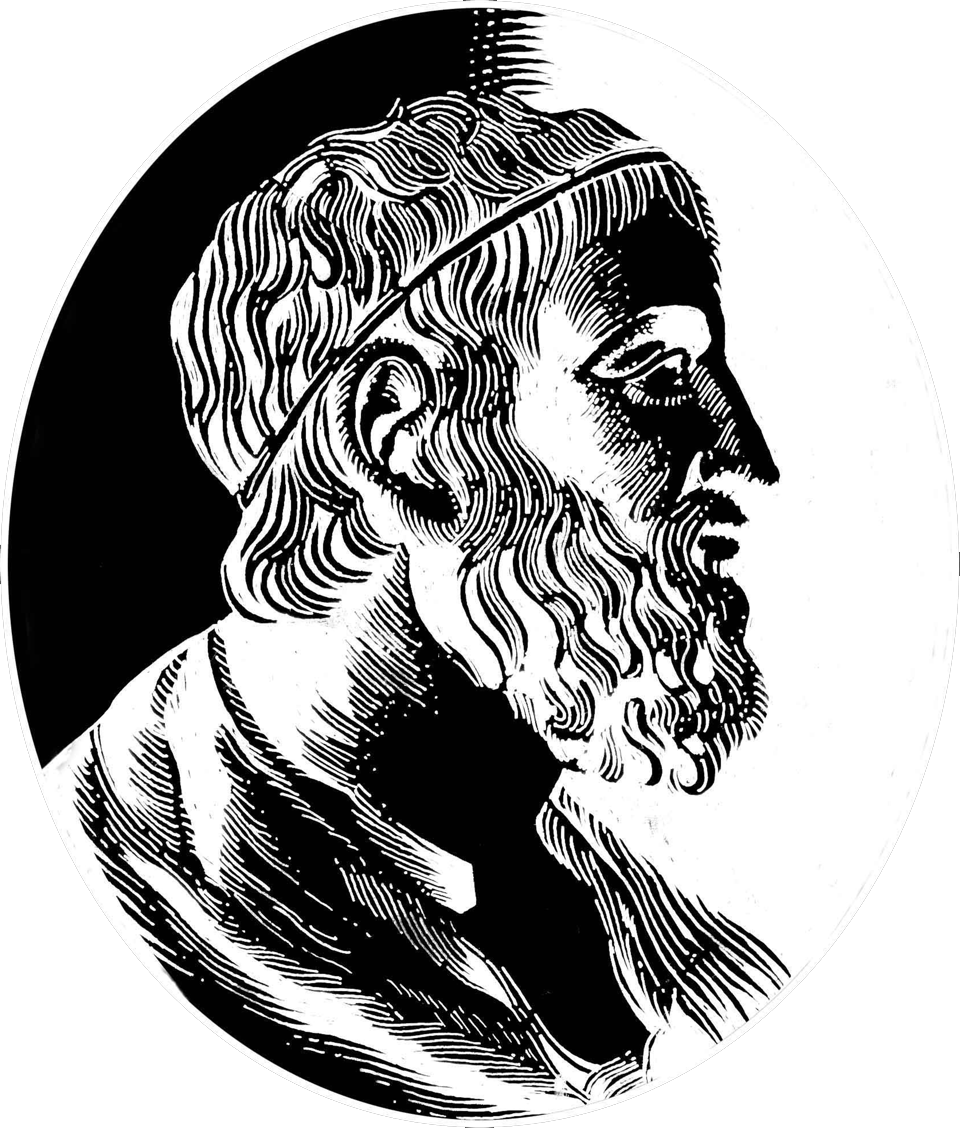
\includegraphics[height=2cm]{imelogo}\\[0.2cm] Department of Computer Science \\ University of São Paulo}

\begin{document}

\maketitle

%------------------------------------------------------------------------------
\section{Bash Startup Files}
\begin{frame}{Bash sequence}
  \metroset{block=fill}
  \begin{exampleblock}{Read file sequence}
		\begin{enumerate}
			\item \texttt{/etc/profile}
			\item \texttt{\~{}/.bash\_profile}
			\item \texttt{\~{}/.bash\_login}
			\item \texttt{\~{}/.profile}
		\end{enumerate}
	\end{exampleblock}

	\begin{exampleblock}{Considerations}
		\begin{itemize}
			\item Usually, \texttt{\~{}/.bashrc} is loaded by
						\texttt{\~{}/.bash\_profile}
			\item Bash invoked with name \texttt{sh}
		\end{itemize}
	\end{exampleblock}
\end{frame}

%------------------------------------------------------------------------------
\section{Bash Conditional Expressions}
\begin{frame}{Bash Conditiona Expressions}
  \metroset{block=fill}
  \begin{exampleblock}{About}
    \begin{itemize}
      \item Used by the \texttt{[[}, \texttt{[}, or \texttt{test}
			\item \texttt{[} or \texttt{[[}?
			\item There is a large number of comparations available in the bash, we
						just show some of them here
    \end{itemize}
  \end{exampleblock}
\end{frame}
%TODO: Adicionar exemplos de condicionais

%------------------------------------------------------------------------------
\section{Shell Arithmetic}
\begin{frame}{Period (.)}
  \metroset{block=fill}
  \begin{exampleblock}{About}
    \begin{itemize}
      \item The operators and their precedence, associativity, and values are
						the same as in the C Language
			\item Operators: id++, id--, ++id, --id, -, +, !, \~{}, **, *, /, \%, >>,
						<<. <=, >=, <, >, ==, !=, \&, \^{}, |, \&\&, ||, expr ? expr : expr,
						=, *=, /=, \%=, +=, -=, <<=, >>=, \&=, \^{}=, |=
    \end{itemize}
  \end{exampleblock}
\end{frame}

%------------------------------------------------------------------------------
\section{Arrays}
\begin{frame}{Arrays}
  \metroset{block=fill}
  \begin{exampleblock}{About}
    \begin{itemize}
      \item Explicit Array: \texttt{declare -a name}
			\item Associative Arrays: \texttt{declare -A name}
			\item Assign value:
			\begin{itemize}
				\item \texttt{name=(value1 value2 value3}
				\item \texttt{name[1]="value"}
				\item \texttt{name["key"]=33}
			\end{itemize}
			\item Get a value: \texttt{\$\{name[index]\}}
			\item Get all values: \texttt{\$\{name[@]\}} or \texttt{\$\{name[*]\}}
			\item Get all keys: \texttt{\$\{!name[@]\}} or \texttt{\$\{!name[*]\}}
			\item Remove one element: \texttt{unset \$\{name[index]\}}
    \end{itemize}
  \end{exampleblock}
\end{frame}
%------------------------------------------------------------------------------
\section{The Directory Stack Builtins}
\begin{frame}{Directory Stack Builtins}
  \metroset{block=fill}
	\begin{alertblock}{Syntax}
		\texttt{dirs [-clpv] [+N | -N] } \\
		\texttt{popd [-n] [+N | -N] } \\
		\texttt{dirs [-n] [+N | -N | dir] }
	\end{alertblock}
\end{frame}

%------------------------------------------------------------------------------
\section{About this presentation}
\begin{frame}[standout]
  % TODO: Improve it
   \begin{center}\ccbysa\end{center}
\end{frame}

%TODO: Bibliography
% break [n]: http://tldp.org/LDP/abs/html/loopcontrol.html
% continue [n]: http://tldp.org/LDP/abs/html/loopcontrol.html
% exec: http://wiki.bash-hackers.org/commands/builtin/exec
% caller: http://wiki.bash-hackers.org/commands/builtin/caller
% key num code: http://invisible-island.net/xterm/xterm-function-keys.html
\maketitle

\end{document}
